\documentclass[a4paper, 12pt]{exam}

%\usepackage{mathpazo}
\usepackage[onehalfspacing]{setspace}
\usepackage{graphicx}
\usepackage{amsmath, amssymb, amsfonts}
\usepackage[table]{xcolor}
\usepackage{gensymb}
\usepackage[]{booktabs}
\usepackage[utf8]{inputenc}
\usepackage{array}
\usepackage{setspace}
\usepackage{xhfill}
\usepackage{enumitem}
\usepackage{multicol}
\usepackage{mathtools}
%\usepackage{background} %Package for adding a watermark

%\backgroundsetup{scale = 1, angle = 0, firstpage = false, opacity=0.1, contents=\includegraphics{Watermark}}

\newcommand{\dho}{\partial}
\newcommand{\cuspac}{\hspace{0.5cm}}
\newcommand{\longspac}{\hspace{1cm}}
\newcommand{\tripdot}{\cdot \cdot \cdot}


\mathtoolsset{showonlyrefs}

\title{
	{Answers to OBC Subsystem Test} \\
	\textbf{\large Team Anant Recruitment Test}\\
	\vspace{0.75cm}
	%\includegraphics[scale = 0.5]{Watermark}
}
\date{28th January, 2024}
\author{Pranav Chandra N.V \\ 2023AAPS0013P}

\begin{document}
	\maketitle
	\newpage
	
	\begin{questions}
		{\large \question \textbf{Landing on ISS}}
		\begin{parts}
			\part \textbf{Diagram of Parts}\\
			An important part of this question is that \textit{UART cannot be used}. This is because both the UART system allows only 1 master and 1 slave, preventing us from using multiple sensors and devices.
			
			Between SPI and I2C, I personally prefer I2C due to the harsh operating environment (of space). I2C possesses an ACK(acknowledge) bit to allow for error checking. As such, the following would be the diagram. Additionally, connection between the processor and memory should be done via UART.
			\begin{figure}[h!]
				\centering
				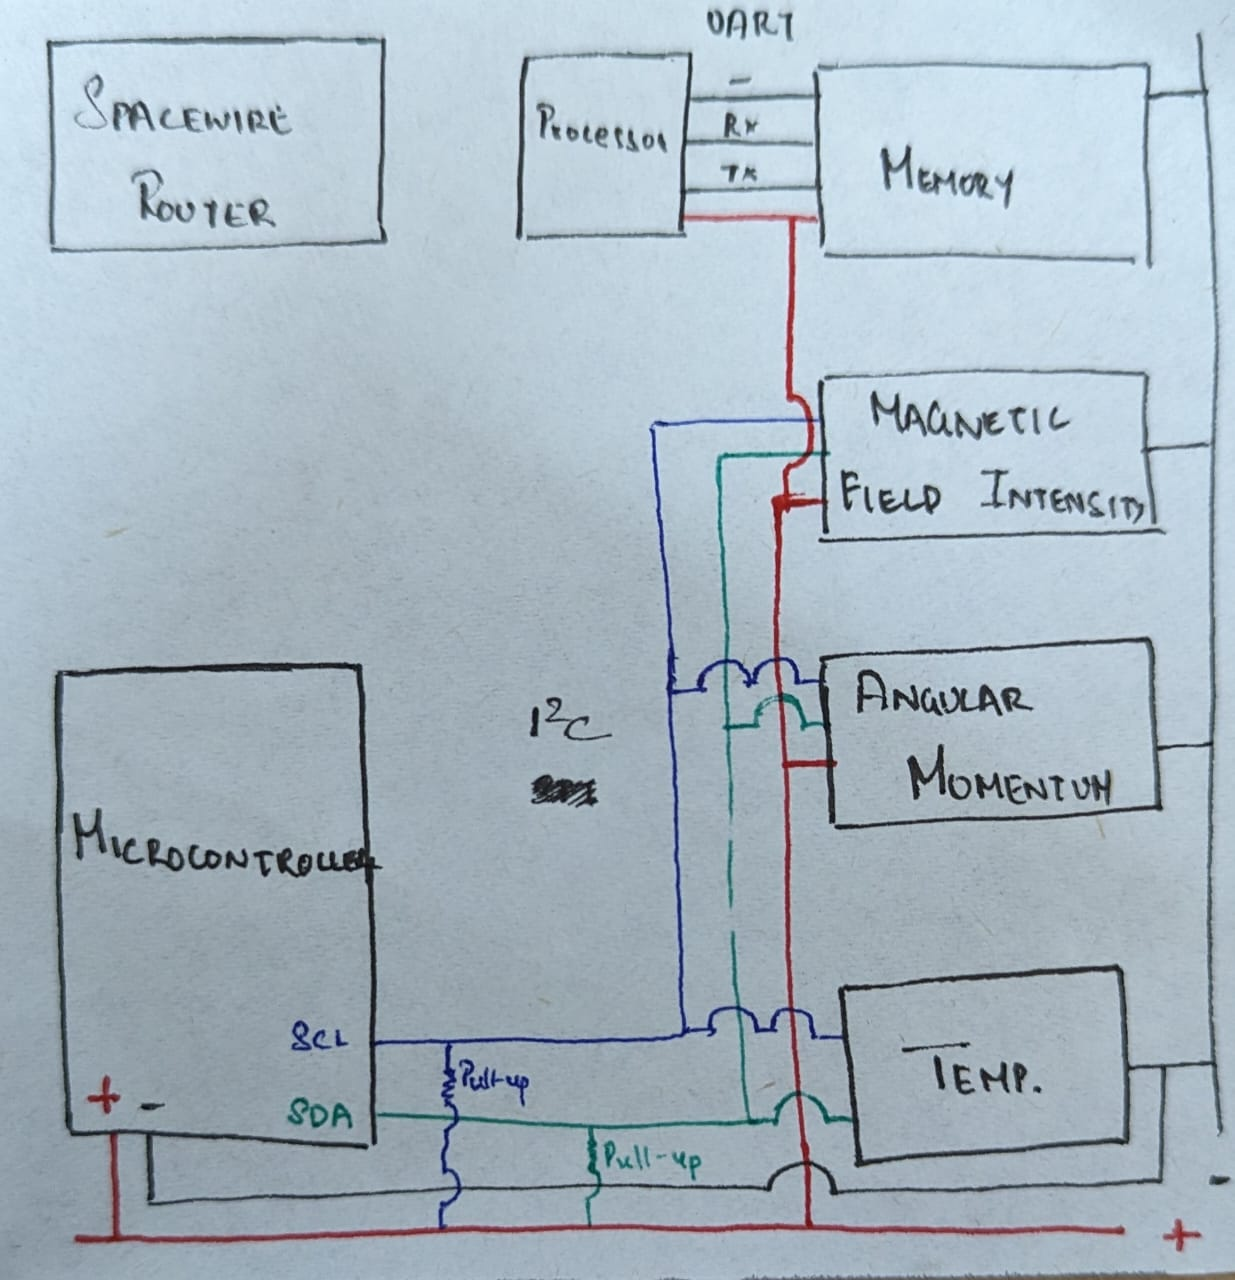
\includegraphics[scale =0.12]{OBC_Q1_Image1}
			\end{figure}
			
			\part \textbf{Connection to Spacewire}
		
			Looking at the documentation (specifically page 18), it looks like spacewire uses a very similar protocol to I2C, intially sending a syncronization bit before sending data across the wire. 
			
			Since I2C has the synchronization as pulling both the SCL and SDA pins high, we can connect the $S_{in}+$ to the SDA/SCL pins. This will trigger the synchronization of the router with the micro controller. We can subsequently send/recieve data over the 4 data pins, $D_{in}+, D_{in}-,D_{out}+, D_{out}-$.
			
			This means that our final connections will look something like this:
			
			\begin{figure}[h!]
				\centering
				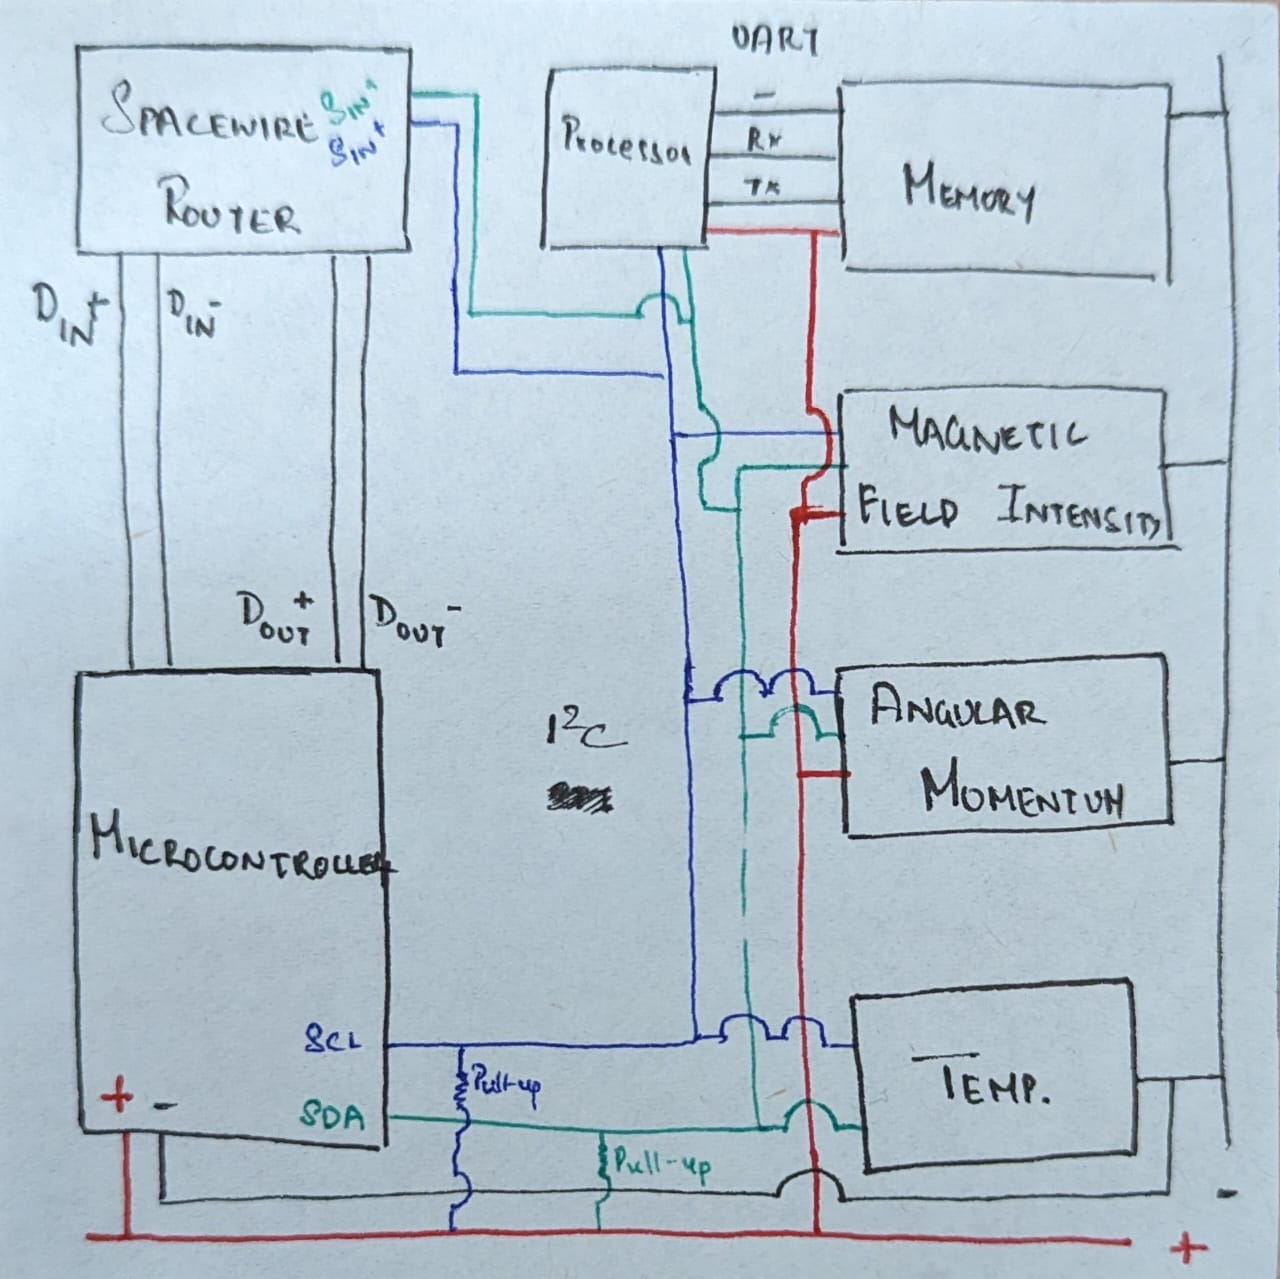
\includegraphics[scale=0.11]{OBC_Q1_Image2}
			\end{figure}
		\end{parts}
	\end{questions}
\end{document}
